\documentclass[12pt,a4paper]{report}

\usepackage[utf8]{inputenc}
%\usepackage[greek,english]{babel}
\usepackage[spanish]{babel}
\usepackage{alphabeta} 

\usepackage[pdftex]{graphicx}
\usepackage[top=1in, bottom=1in, left=1in, right=1in]{geometry}
\usepackage{caption,subcaption}

\linespread{1.06}
\setlength{\parskip}{8pt plus2pt minus2pt}

\widowpenalty 10000
\clubpenalty 10000

\newcommand{\eat}[1]{}
\newcommand{\HRule}{\rule{\linewidth}{0.5mm}}

\usepackage[official]{eurosym}
\usepackage{enumitem}
\setlist{nolistsep,noitemsep}
\usepackage[hidelinks]{hyperref}
\usepackage{verbatim} 
\usepackage{cite}
\usepackage{pgfgantt}
\usepackage{lipsum}


%%%%%%%%%%%%%%%%%%%%%%%%%%%%%%%%%%%%%%%%%%
% Definición del estilo personalizado
\usepackage{listings}
\usepackage{xcolor}

\definecolor{codegreen}{rgb}{0,0.6,0}
\definecolor{codegray}{rgb}{0.5,0.5,0.5}
\definecolor{codepurple}{rgb}{0.58,0,0.82}
\definecolor{backcolour}{rgb}{0.95,0.95,0.92}

\lstdefinestyle{mystyle}{
    backgroundcolor=\color{backcolour},   
    commentstyle=\color{codegreen},
    keywordstyle=\color{magenta},
    numberstyle=\tiny\color{codegray},
    stringstyle=\color{codepurple},
    basicstyle=\ttfamily\footnotesize,
    breakatwhitespace=false,         
    breaklines=true,                 
    captionpos=b,                    
    keepspaces=true,                 
    numbers=left,                    
    numbersep=5pt,                  
    showspaces=false,                
    showstringspaces=false,
    showtabs=false,                  
    tabsize=2
}
%%%%%%%%%%%%%%%%%%%%%%%%%%%%%%%%%%%%%%%%%%


\usepackage{amsmath}
\usepackage{listings}
\usepackage{float}
\usepackage{geometry}
\geometry{verbose,a4paper,tmargin=2.5cm,bmargin=2.5cm,lmargin=2.5cm,rmargin=2.5cm}
\usepackage{hyperref}
\usepackage{xcolor}
\hypersetup{
    colorlinks,
    linkcolor={blue!80!},
    citecolor={blue!80!},
    urlcolor={blue!80!}
}


\begin{document}

\begin{titlepage}
\centering
{
\includegraphics[width=0.2\textwidth]{./img/logo}\par}
\vspace{0.5cm}
{\bfseries\LARGE Universidad de Alcalá  \par}
\vspace{0.4cm}
{\scshape\Large Escuela Politécnica Superior \par}
\vspace{1.2cm}
{\bfseries\Large MÁSTER UNIVERSITARIO EN INGENIERÍA DE TELECOMUNICACIÓN  \par}
\vspace{2.1cm}
{\scshape\Huge Práctica Entregable 1 \\ Transmisor 16 QAM\par}
\vspace{1.5cm}
{\itshape\Large Diseño de Circuitos Electrónicos para Comunicaciones \par}
\vfill
{\Large Autor: \par}
{\Large Paula Bartolomé Mora \par}
\vfill
{\Large \today \par}
\end{titlepage}

\newpage

%===========================================================
\tableofcontents
\addtocontents{toc}{\protect\thispagestyle{empty}}
\newpage
\setcounter{page}{1}

%===========================================================
%===========================================================

\chapter{Introducción}
\label{section:intro}

El presente trabajo tiene como objetivo principal el desarrollo de un sistema de comunicaciones basado en 16-QAM (Modulación de Amplitud en Cuadratura de 16 niveles). Para ello, se propone el empleo en conjunto de los diferentes bloques electrónicos IP estudiados en la asignatura y se divide el desarrollo del entregable en una serie de fases de configuración:

\vspace{1mm}

\begin{itemize}
    \item \textbf{Captura XADC y Memoria FIFO:} En esta primera etapa se realizará la captura de una señal triangular y se procederán a almacenar los datos de entrada en una memoria FIFO.
    \item \textbf{Mapeado QAM y Zero Padding: } Como siguiente paso a seguir, se generará el mapeado de 16-QAM y se implementará un Zero-Padding 1:32. 
    \item \textbf{Filtrado Root Raised Cosine: } Tras aplicar Zero Padding, se deberá generar y aplicar a cada rama I/Q el filtrado pulse shaping del “root raised cosine” (RRC).
    \item \textbf{Mezclador DDS y Multiplicadores: ----------}
    \item \textbf{Sumador: ----------}
    \item \textbf{Rx: ----------}

    
\end{itemize}

\vspace{3mm}

    \begin{figure}[h]
    	\centering
    	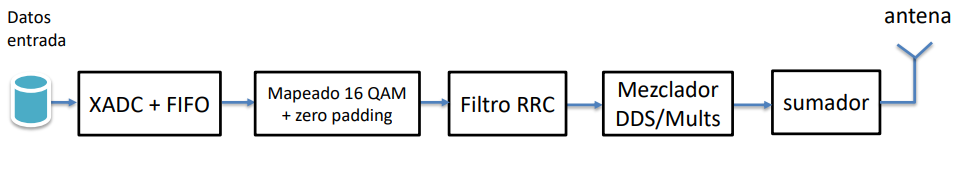
\includegraphics[width=1\textwidth]{img/diseno/sistema.PNG}
    	\caption{Distribución de bloques del sistema de comunicaciones}
    	\label{fig:sistema}
    \end{figure}
    
\vspace{3mm}

Para lograr tanto un correcto funcionamiento de cada bloque electrónico como la interoperabilidad entre ellos al integrarlos en del sistema, será preciso un estudio en profundidad de la documentación proporcionada por el fabricante y un análisis cuantitativo y cualitativo de cada uno de los resultados obtenidos en las simulaciones funcionales. 

\vspace{1mm}

%Finalmente, se deberá evaluar la eficacia de la modulación 16-QAM en la transmisión de datos
%Se adjunta el enunciado en archivo pdf y un archivo de matlab "qam16.m" para simular el funcionamiento de la transmisión de datos usando 16QAM.


%1.	Obtención de los datos convertidos del ADC – simulación señal de entrada 
%2.	Lógica de control de lectura/escritura de los datos de la FIFO. Comprobación del bloque FIFO 
%3.	Bloque de mapeado 16QAM y zero-padding 
%4.	Bloque de filtrado pulse shaping - RRC 
%5.	Generación de las sinusoides coseno/-seno mediante bloque DDS a 576 MHz 
%6.	Bloque de multiplicación y suma de señales de transmisión I/Q. Comprobación de datos. 
%7.	Configuración y uso del bloque MMCM en el diseño 
%8.	Codificación de ficheros testbench y pruebas realizadas para la verificación del funcionamiento junto con el simulador Matlab. 
%9. Realización de un diseño modular que funcione correctamente en su conjunto 
%10. Inclusión de otras alternativas/opciones adicionales en el diseño planteado






\chapter{Captura XADC y memoria FIFO}
\label{section:xadc_fifo}


Como se ha introducido anteriormente, en este capítulo se definirá el proceso de captura y conversión de una señal de entrada triangular y el posterior almacenamiento de la misma en una memoria FIFO. En la Figura \ref{fig:xadc_fifo} se muestra el diseño de los bloques necesarios para esta fase y la definición de sus correspondientes puertos de entrada y salida.

\vspace{3mm}

    \begin{figure}[h]
    	\centering
    	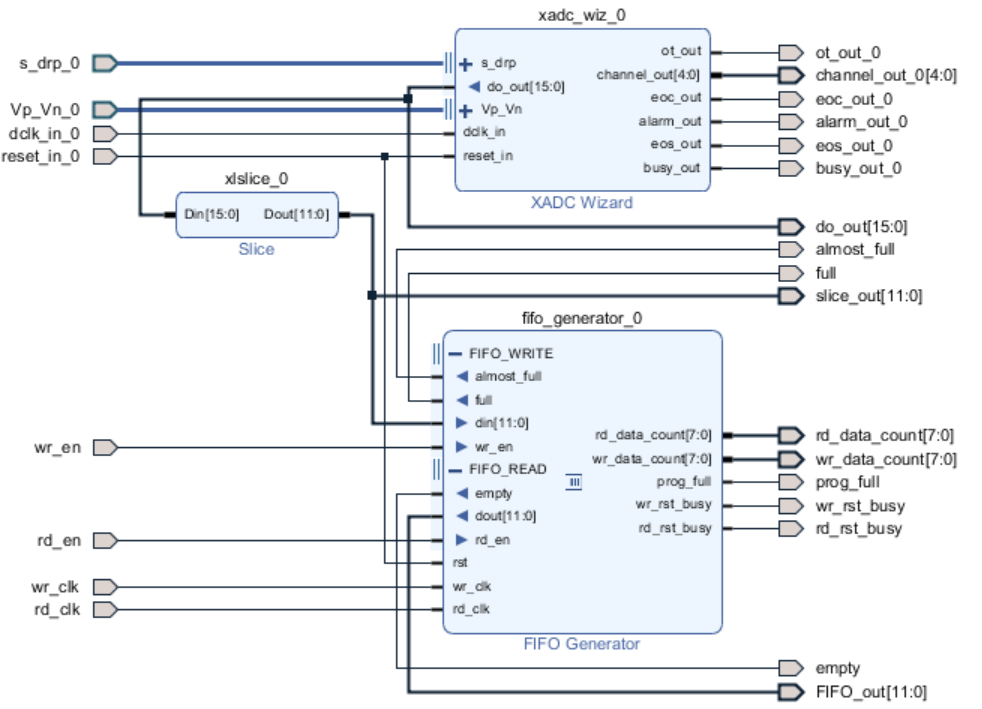
\includegraphics[width=1\textwidth]{img/diseno/xadc_fifo.PNG}
    	\caption{Diseño del bloque XADC+FIFO}
    	\label{fig:xadc_fifo}
    \end{figure}
    
\vspace{3mm}

\section{Obtención de los datos convertidos del ADC}

\subsection{Configuración del XADC}

En primer lugar, teniendo en cuenta que nuestro puesto de laboratorio es el 8, se debe generar a la entrada una señal triangular con un valor de frecuencia igual a 13KHz y que opere en un rango de valores de tensión entre 0 y 0.596 voltios. Los valores que toma en cada instante temporal serán definidos en el fichero design.txt, el cual tendrá que ser importado al proyecto para llevar a cabo la conversión.

Como se puede ver en la Figura \ref*{fig:design} se definen valores de tensión para dos entradas (VP y VN), que corresponden a las entradas analógicas diferenciales del XADC. Por simplificación, se configura el valor absoluto de tensión para la entrada positiva (VP) y un valor nulo para la negativa (VN). 

\vspace{3mm}

    \begin{figure}[h]
    	\centering
    	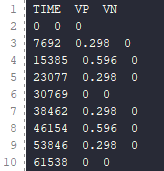
\includegraphics[width=0.3\textwidth]{img/diseno/design.PNG}
    	\caption{Valores de tensión (V) de la señal triangular extraídos de design.txt}
    	\label{fig:design}
    \end{figure}
    
\vspace{3mm}

%el escalon max del ADC = (3/4096)/2 -> el error max, la precisión tiene que ser menor que el error, si no se pierde resolución.
%en vp_vn se pone una precisión segun esto
%0.000366 -> precisión de 10e-4, tensiones de 4 decimales.

El XADC se configura en modo continuo y con un único canal de entrada para capturar las muestras, por lo que se ha seleccionado el canal 3 para registrar el valor convertido de tensión (\textit{s\_drp\_daddr}). La conversión se realizará a una velocidad de 1 MS/seg con un reloj de 52 MHz y se establecerá un tiempo de adquisición igual a 4 para que la señal de captura sea estable.

%hablar de la configuración del xadc
%poner foto del esquema de la documentación
%hablar del 192mhz



\subsection{Simulación de la señal de entrada}

Una vez configurado el bloque IP XADC se procede a simular la conversión de la señal de entrada. En la figura \ref{fig:xadc} se puede visualizar cómo se obtiene la salida digital de 16 bits por el puerto \textit{do\_out}.

\vspace{3mm}

\begin{figure}[h]
    \centering
    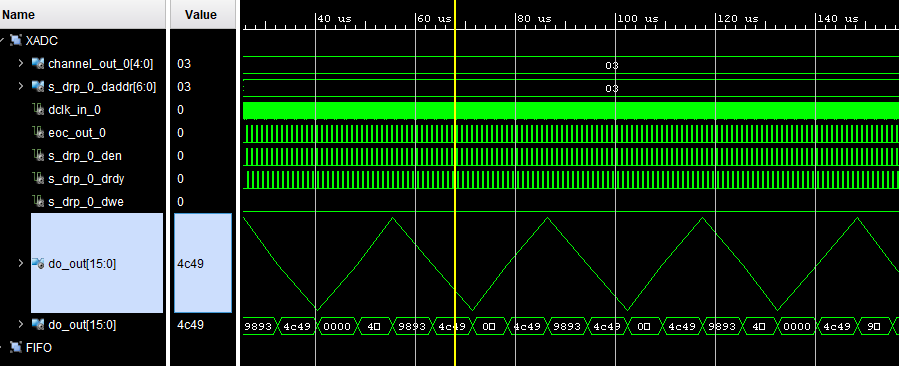
\includegraphics[width=1\textwidth]{img/simu/xadc.PNG}
    \caption{Conversión analógico-digital de la señal triangular de entrada (I)}
    \label{fig:xadc}
\end{figure}

\vspace{3mm}

Por otro lado, en la Figura \ref{fig:xadc2} se aprecia de una forma más clara los valores que toman cada uno de los puertos del XADC en cada conversión. La señal de fin de conversión \textit{eoc\_out} se activa y como consecuencia, también lo hará la de enable del Puerto de Reconfiguración Dinámico (DRP) \textit{eoc\_out}. La operación de lectura se completa cuando la señal de dato ready se activa \textit{s\_drp\_drdy}, indicando que se ha sacado el dato a la salida y que se puede proceder a convertir el siguiente.

\vspace{3mm}

\begin{figure}[h]
    \centering
    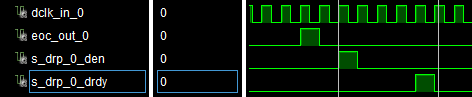
\includegraphics[width=0.7\textwidth]{img/simu/xadc2.PNG}
    \caption{Fin de conversión y dato preparado (III)}
    \label{fig:xadc2}
\end{figure}

\vspace{3mm}

\section{Lógica de control de lectura y escritura de los datos de la FIFO}

\subsection{Configuración del bloque FIFO}

El bloque de memoria FIFO almacenará cada uno de los datos capturados por el bloque XADC. Consta de una capacidad de 256 posiciones de 12 bits cada una, por lo que a la entrada del bloque FIFO será precisa la configuración de un bloque auxiliar Slice para transformar los 16 bits de la señal de salida del XADC en sus 12 bits de mayor peso. Además, esto es necesario porque el XADC en el fondo maneja una precisión de 12 bits a la salida. 

Cada vez que exista un nuevo dato proporcionado por el XADC se escribirá en la memoria FIFO de forma continua a 1 MS/s y con un reloj de 52 MHz (\textit{wr\_clk}) hasta llegar a la capacidad máxima. Una vez la memoria FIFO está llena, comenzará el proceso de lectura de 200 datos a una frecuencia de lectura de 2MHz (\textit{rd\_clk}). En este caso, al desear leer un número de datos menor a la capacidad máxima (256), será necesario configurar una señal auxiliar programable (\textit{programable\_full}).

\vspace{3mm}

    \begin{figure}[h]
    	\centering
    	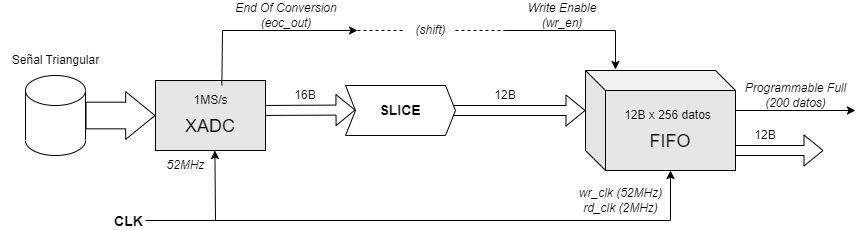
\includegraphics[width=1\textwidth]{img/diseno/xadc_fifo.drawio.PNG}
    	\caption{Diseño del bloque XADC+FIFO}
    	\label{fig:xadc_fifo}
    \end{figure}
    
\vspace{3mm}

\subsection{Comprobación del bloque FIFO}

%explicar como esta relacionado con el xadc
%configuración de contadores de lectura y escritura
      
       % for i in 0 to 200 -- a la espera de 200 datos 
        %loop     
        %    dato_i <= i;
\chapter{Modulador 16-QAM}
\label{section:qam}


En este Capítulo se muestra el bloque encargado de la modulación 16-QAM. Este bloque se compone de tres procesos: mapeado 16-QAM, aplicación de Zero Padding y filtrado \textit{Root Raised Cosine}. En la Figura \ref{fig:qam_fir} se puede visualizar la estructura de los bloques IP que se han incluido en este segundo proyecto de Vivado. 

\vspace{1mm}

\begin{figure}[h]
	\centering
	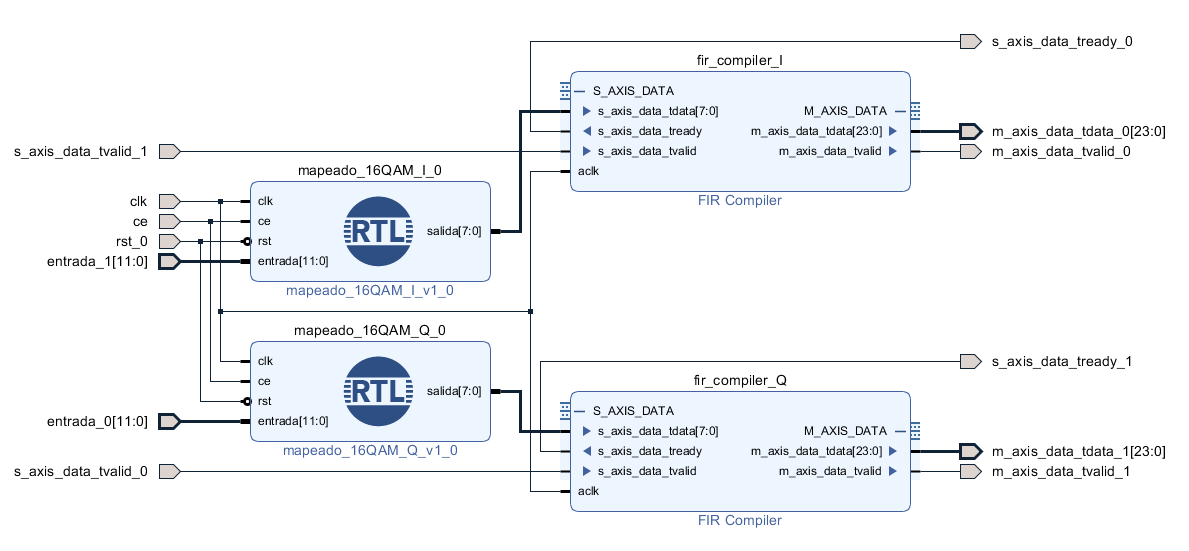
\includegraphics[width=1\textwidth,height=9cm]{img/diseno/qam_fir.PNG}
	\caption{Diseño de los bloques mapeado 16-QAM + ZP y filtrado RRC}
	\label{fig:qam_fir}
\end{figure}
    
\vspace{1mm}

\section{Mapeado 16-QAM}

\subsection{Configuración del mapeado 16-QAM}

Para implementar una modulación 16-QAM (Modulación de Amplitud en Cuadratura) lo primero que se debe realizar es el bloque de mapeado, con el fin de asignar patrones de amplitud y fase a cada símbolo y proporcionar una mayor eficiencia espectral. 

\vspace{3mm}

Para ello, se recibe una señal de entrada de 12 bits, obtenida a partir de la lectura de los 200 valores almacenados en la memoria FIFO. Se debe crear un proceso en el testbench que se ejecute en cada ciclo del reloj global, configurado a 192MHz, que realice la lectura del fichero \textit{FIFO\_out.txt}. Como se había descrito en el Apartado \ref{section:fifo}, se escriben en dicho fichero los valores almacenados en la memoria FIFO para emplearlo como la entrada del bloque de mapeado 16-QAM y optimizar así los proyectos de Vivado.

\vspace{5mm}

\begin{lstlisting}[language=VHDL, style=mystyle, caption={Proceso de lectura del fichero FIFO\_out.txt}]
	process(clk) --192MHz
    variable line_buffer : line;
    variable nuevo_valor : STD_LOGIC_VECTOR(11 DOWNTO 0);
    
    begin
        if rst_0 = '1' then
            eof <= false; --se reinicia fin de archivo
            cont_in <= 0;
        elsif rising_edge(clk) then
            cont_in <= cont_in + 1;
            if cont_in = 96 then --cada 500 ns se lee entrada
                cont_in <= 0;
                if not eof then
                    if endfile(file_handle) then 
                        eof <= true; 
                    else
                        readline(file_handle, line_buffer);
                        read(line_buffer, nuevo_valor);
                        entrada <= nuevo_valor;
                    end if;
                end if;
            end if;                      
        end if;
end process;  
\end{lstlisting}

\vspace{2mm}

Es importante tener en cuenta que la lectura se produce a una frecuencia de 2MHz, por lo que se debe añadir un contador de 96 ciclos en el proceso, además de comprobar si el fichero ha llegado al final. Según las especificaciones de este proyecto, la salida del mapeado debe funcionar a una frecuencia de 6MHz, es decir, el triple de la anterior porque por cada valor a la entrada de 12 bits se obtendrán 3 símbolos 16-QAM. En otros términos, se tratarán los bits de entrada de 4 en 4 para mapear cada símbolo 16-QAM. 

El mapeado de cada símbolo 16-QAM supone la generación a la salida de dos caminos independientes: uno para la componente en Fase (I) y otro para la de Cuadratura (Q). Cada símbolo es de 3 bits con signo y puede tomar los valores (-3,-1,+1,+3) como se puede visualizar en la Figura \ref{fig:qam}, procedente del ejemplo simulado en Matlab.

\vspace{3mm}

\begin{figure}[h]
	\centering
	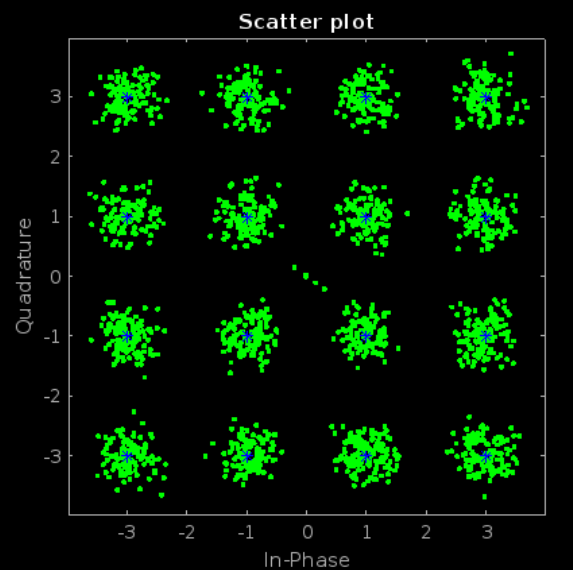
\includegraphics[width=0.4\textwidth]{img/matlab/qam.PNG}
	\caption{Constelación 16-QAM}
	\label{fig:qam}
\end{figure}

\vspace{3mm}
   
En este caso, se han decidido ajustar las tablas Q e I para establecer una codificación Gray. Esta se trata de una técnica específica que garantiza que solo un bit cambie entre dos valores consecutivos. Además, consigue minimizar la posibilidad de errores producidos por cambios de múltiples bits en la transmisión. A continuación, se puede visualizar la definición de cada una de las tablas:

\vspace{4mm}

\begin{lstlisting}[language=VHDL, style=mystyle, caption={Definición de la tabla de mapeado Q}]
type Array3Bit is array (0 to 15) of STD_LOGIC_VECTOR(2 downto 0);
constant tabla_mapeado_Q: Array3Bit :=
		("000", "001", "011", "010", 
		"110", "111", "101", "100",
		"000", "001", "011", "010", 
		"110", "111", "101", "100");
\end{lstlisting}

\vspace{5mm}

\begin{lstlisting}[language=VHDL, style=mystyle, caption={Definición de la tabla de mapeado I}]
type Array3Bit is array (0 to 15) of STD_LOGIC_VECTOR(2 downto 0);
constant tabla_mapeado_I: Array3Bit := 
	("000", "000", "001", "001", 
	"011", "011", "010", "010",
	"110", "110", "111", "111", 
	"101", "101", "100", "100");
\end{lstlisting}

\pagebreak

\section{Proceso de mapeado + Zero Padding}

\subsection{Configuración del proceso de mapeado + Zero Padding}

Además de implementar el mapeado 16-QAM, se añade en el bloque el zero-padding para optimizar el sistema de comunicación. Se insertan ceros a la señal original y se extiende su duración, aplicando en este caso una relación 1:32. Por lo tanto, por cada flanco en el que se transmita información, le seguirán 31 flancos en los que se transmitan bits con valor cero.

Siguiendo las especificaciones anteriores, se decide combinar el mapeado 16-QAM con el zero-padding en un mismo bloque, para así obtener a la salida del mismo los símbolos 16-QAM con el Zero Padding ya aplicado. Así, se garantiza que la señal tenga una duración suficiente para conseguir una respuesta de frecuencia óptima, además de minimizar la interferencia entre símbolos. De forma adicional, se ajusta la salida a una longitud de 8 bits para dejarla preparada para la entrada del filtro pulse shaping del \textit{Root Raised Cosine} (RRC). 

\vspace{3mm}

\begin{lstlisting}[language=VHDL, style=mystyle, caption={Proceso de mapeado (Camino I) + Zero Padding}]
process(clk) 
	variable contador : integer := 0; -- 4*contador+3 downto 4*contador
	variable cont_32 : integer := 0; -- 6MHz
	variable captured_bits : std_logic_vector(3 downto 0) := "0000";
	variable aux_salida : std_logic_vector(2 downto 0):= "000";
begin
	if rising_edge(clk) then
		if rst = '1' then
			contador := 0; 
			cont_32 := 0; 
			salida <= (others => '0'); 
		else
			if cont_32 = 32 then -- se saca simbolo por la salida
				cont_32 := 0;
				captured_bits := entrada(4*contador+3 downto 4*contador);
				aux_salida := tabla_mapeado_I(to_integer(unsigned(captured_bits))); 
				--salida extendida a 8 bits
				salida(2 downto 0) <= aux_salida; 
				salida(7 downto 3) <= (others => aux_salida(2));
				contador := contador + 1; 
				if contador = 3 then 
					contador := 0; 
				end if;
			else --Zero Padding
				cont_32 := cont_32 + 1;
				salida <= (others => '0');
			end if;
		end if;
	end if;         
end process; 
\end{lstlisting}

\pagebreak

Como se puede visualizar, el proceso emplea dos contadores: uno para extraer en cada flanco los bits capturados de 4 en 4 e implementar el mapeado QAM para obtener los símbolos de 3 bits y otro, para implementar la relación 1:32 respectiva al Zero Padding.

\subsection{Comprobación del proceso de mapeado + Zero Padding}
\label{sec:map}

En el testbench se incluye el proceso de estimulación de las señales de habilitación (\textit{clock enable}) y de reset del bloque de mapeado. También, se pueden apreciar las líneas de código dedicadas a la activación de las señales de validación de datos del filtro (\textit{s\_axis\_data\_tvalid}), pero esto se detallará en el Apartado \ref{sec:fir}. 

\vspace{3mm}

Además, se deben abrir los ficheros correspondientes a la lectura y escritura de datos para cada uno de los bloques: para lectura de las muestras almacenadas en la FIFO y para escritura de las salidas de las ramas de filtrado.

\vspace{3mm}

\begin{lstlisting}[language=VHDL, style=mystyle, caption={Proceso de estimulación de señales de reset y clock enable}]
process
begin
   file_open(file_handle, ".\FIFO_output.txt", READ_MODE);
   file_open(file_handle_I, ".\FIR_output_I.txt", WRITE_MODE);
   file_open(file_handle_Q, ".\FIR_output_Q.txt", WRITE_MODE);
	
   ce <= '0';
   rst_0 <= '1';        
  
   s_axis_data_tvalid_0 <= '0';
   s_axis_data_tvalid_1 <= '0';
	
   wait for 32*clk_period;
   rst_0 <= '0';

   wait for 32*clk_period;
   ce <= '1';
   s_axis_data_tvalid_0 <= '1';
   s_axis_data_tvalid_1 <= '1';  
		  
   wait;
end process;  
\end{lstlisting}

\vspace{3mm}

A continuación, en las Figuras \ref{fig:proc2}, \ref{fig:proc3} y \ref{fig:proc1} se puede apreciar cómo se implementa el bloque de mapeado 16-QAM + zero-padding a través del proceso expuesto anteriormente.

\begin{sidewaysfigure}
	\centering
	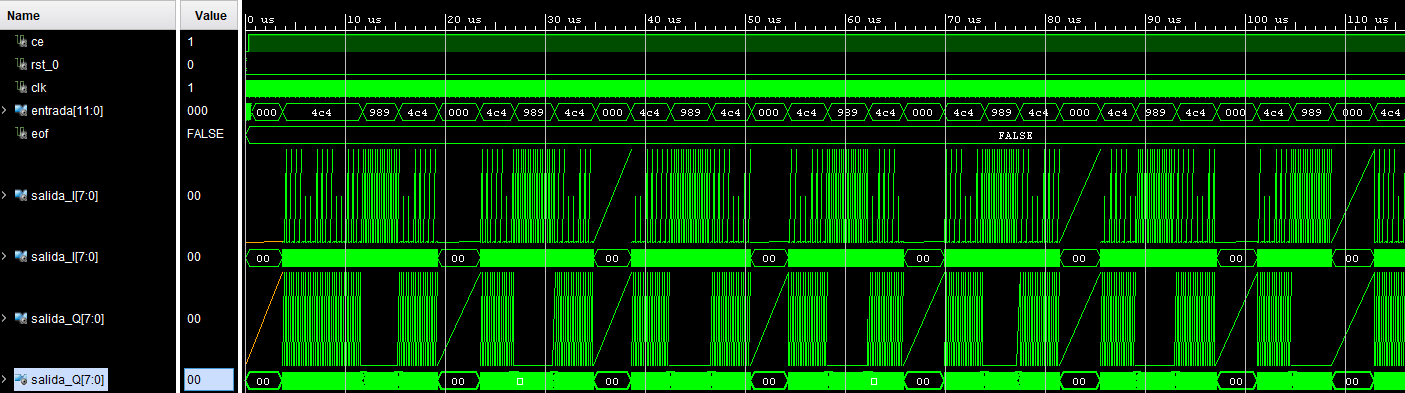
\includegraphics[width=1\textwidth, height=7cm]{img/simu/process_qam_2.PNG}
	\caption{Simulación completa del proceso de mapeado 16-QAM + ZP}
	\label{fig:proc2}
\end{sidewaysfigure}

\clearpage

\begin{sidewaysfigure}
	\centering
	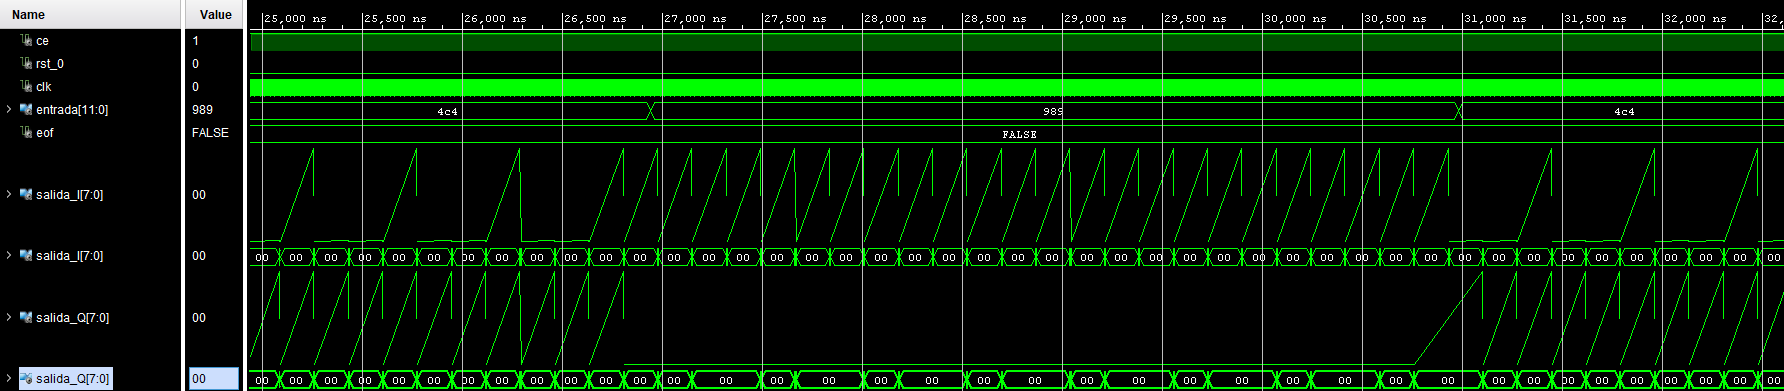
\includegraphics[width=1\textwidth, height=7cm]{img/simu/process_qam_3.PNG}
	\caption{Simulación del proceso de mapeado 16-QAM + ZP (II) (zoom medio)}
	\label{fig:proc3}
\end{sidewaysfigure}

\clearpage

\begin{sidewaysfigure}
	\centering
	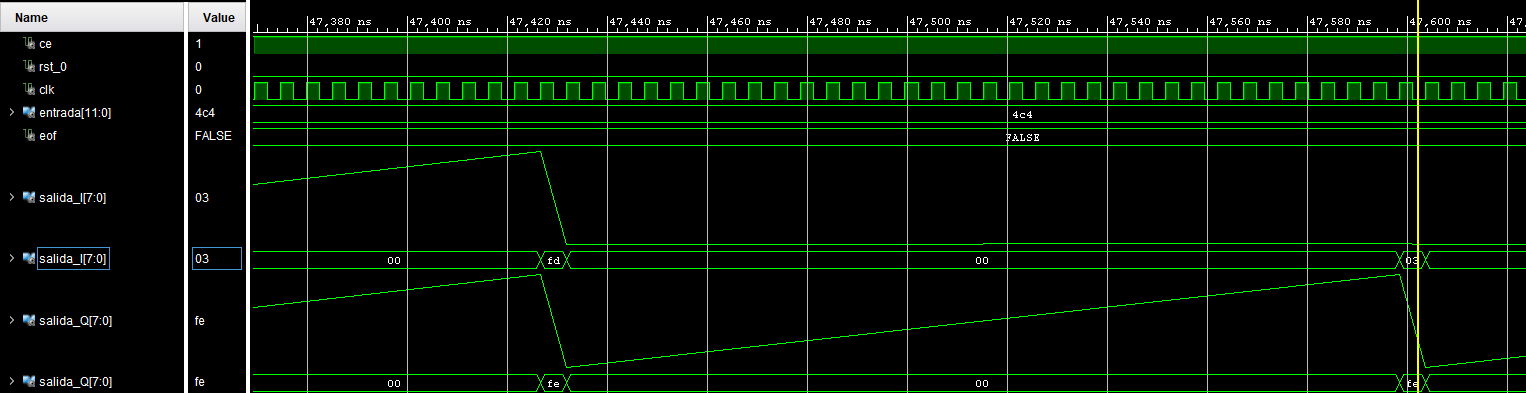
\includegraphics[width=1\textwidth, height=7cm]{img/simu/process_qam.PNG}
	\caption{Simulación del proceso de mapeado 16-QAM + ZP (III) (zoom alto)}
	\label{fig:proc1}
\end{sidewaysfigure}

\clearpage

\section{Bloque de filtrado pulse shaping - RRC}

\subsection{Configuración del filtro RRC}

El filtro pulse shaping del \textit{Root Raised Cosine} (RRC) es un tipo de filtro denominado de coseno elevado. Se emplea en sistemas de comunicación digital para dar forma de onda a los pulsos que se transmiten. Minimiza la interferencia entre símbolos adyacentes y maximiza la eficiencia del espectro.

\vspace{3mm}

El primer paso a seguir para crear el filtro RRC es obtener los coeficientes del mismo. Para ello, se va a emplear Matlab, estableciendo de la siguiente forma las especificaciones del filtro a diseñar:

\vspace{5mm}

\begin{lstlisting}[language=matlab, style=mystyle, caption={Diseño del filtro RRC en Matlab}]
filtlen = 6;      % Longitud del filtro en numero de simbolos
rolloff = 0.25;   % Factor de rolloff para controlar el ancho del pulso
sps = 32;         % Muestras por simbolo (factor de oversampling)

rrcFilter = rcosdesign(rolloff,filtlen,sps);
fvtool(rrcFilter,'Analysis','Impulse')
\end{lstlisting}

\vspace{3mm}

Tras ejecutar el código, se obtendrán en total 193 coeficientes. Esto tiene como consecuencia que, para aplicar el filtro a la señal de entrada se irá ajustando un enventanado de longitud igual a 193 datos (dato actual + 192 datos siguientes) hasta finalizar la etapa. 

\vspace{3mm}

\begin{figure}[h]
	\centering
	\includegraphics[width=1\textwidth]{img/matlab/rrc.PNG}
	\caption{Respuesta al impulso del filtro RRC}
	\label{fig:fvtool}
\end{figure}
    
\vspace{3mm}

Mediante la herramienta gráfica \textit{fvtool} que proporciona Matlab se puede obtener la respuesta impulsiva del filtro RRC tal y como se muestra en la Figura \ref{fig:fvtool}.

Para añadir el bloque del filtro en Vivado se requiere conocer el número de bits de los coeficientes, tanto de la parte entera como de la parte fraccionaria. Para ello, se emplea el comando de MatLab \textit{sfi(rrcFilter)} y se obtiene la salida de la Figura \ref{fig:fvtool2}

\vspace{3mm}

\begin{figure}[h]
	\centering
	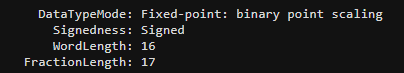
\includegraphics[width=0.6\textwidth]{img/matlab/coefs.PNG}
	\caption{Información sobre la matriz de coeficientes del filtro RRC}
	\label{fig:fvtool2}
\end{figure}
    
\vspace{3mm}

Como los coeficientes se encuentran dentro de un rango de valores entre 0 y 1, se establecen 16 bits para la logitud total y 17 bits, para la parte fraccionaria. Por otro lado, se configura el modo de truncamiento, una salida de filtrado de 24 bits y una entrada de 8 bits, que ya ha sido previamente ajustada en el bloque anterior, por lo que no se requieren procesos adicionales (ver Figura \ref{fig:fvtool3}).

\vspace{3mm}

\begin{figure}[h]
	\centering
	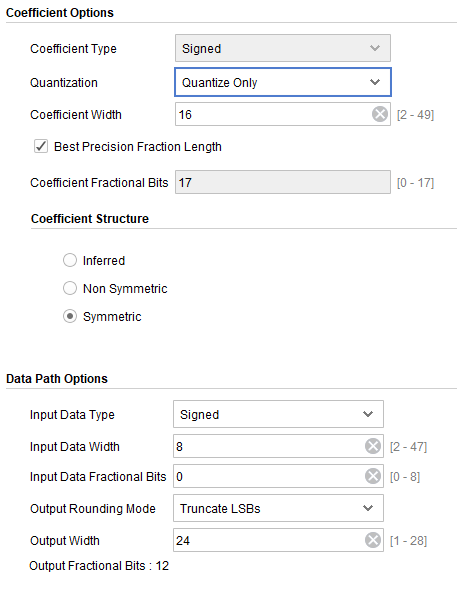
\includegraphics[width=0.6\textwidth]{img/diseno/fir.PNG}
	\caption{Configuración del filtro en Vivado}
	\label{fig:fvtool3}
\end{figure}
    
\pagebreak

Entrando en el código, para que el filtrado comience a operar es necesario primero resetear las entradas de validación de datos \textit{s\_axis\_data\_tvalid} de ambos filtros (camino I y Q) y después, activarlas cuando la señal de \textit{clock enable} se pone a 1. 

Por otro lado, como se había realizado con la salida de la memoria FIFO, para el bloque de filtrado también se van a almacenar los valores de salida en un fichero .txt. Para ello, se emplea el proceso definido anteriormente para la lectura de la FIFO y se añaden las líneas necesarias de escritura de los nuevos ficheros.

\vspace{5mm}

\begin{lstlisting}[language=vhdl, style=mystyle, caption={Proceso de escritura de los ficheros FIR\_output\_I.txt y FIR\_output\_Q.txt}]
process(clk) --192MHz
    --lectura datos FIFO
    variable line_buffer : line;
    variable nuevo_valor : STD_LOGIC_VECTOR(11 DOWNTO 0);
    
    --escritura datos FIR
    variable line_buffer_I, line_buffer_Q : line;
    variable nuevo_valor_I, nuevo_valor_Q : integer;
    
    begin
        if rst_0 = '1' then
            eof <= false; --se reinicia fin de archivo
            cont_in <= 0;
        elsif rising_edge(clk) then
            cont_in <= cont_in + 1;
            if cont_in = 96 then --cada 500 ns se lee entrada 
                cont_in <= 0;
                if not eof then
                    if endfile(file_handle) then 
                        eof <= true; 
                    else
                        readline(file_handle, line_buffer);
                        read(line_buffer, nuevo_valor);
                        entrada <= nuevo_valor;
                    end if;
                end if;
            end if; 
            if s_axis_data_tvalid_0 = '1' and s_axis_data_tvalid_1 = '1' and not eof then 
                --escritura de salida FIR I a 192MHz
                nuevo_valor_I:=to_integer(signed(m_axis_data_tdata_0));
                write(line_buffer_I, nuevo_valor_I); 
                writeline(file_handle_I, line_buffer_I); 
                --escritura de salida FIR Q a 192MHz
                nuevo_valor_Q:=to_integer(signed(m_axis_data_tdata_1));
                write(line_buffer_Q, nuevo_valor_Q); 
                writeline(file_handle_Q, line_buffer_Q);
            end if;                      
        end if;
end process; 
\end{lstlisting}

\pagebreak

\subsection{Comprobación del filtrado RRC}
\label{sec:fir}

En las Figuras \ref{fig:rrc1} y \ref{fig:rrc2} se visualiza la simulación completa del proyecto que incluye los bloques de mapeado 16-QAM + zero-padding y filtrado RRC. Se puede comprobar cómo el filtro da forma de onda a los pulsos que se transmiten y que provienen del proceso de mapeado previo.

Como se había adelantado en el Apartado \ref{sec:map}, en el testbench se deben activar las señales de validación de datos del filtro (\textit{s\_axis\_data\_tvalid}) a la vez que se produce la habilitación del \textit{clock enable} del mapeado. Esto es imprescindible añadirlo para que no se realice el filtrado si no existen nuevas muestras de entrada. 

\vspace{3mm}

\begin{figure}[h]
	\centering
	\includegraphics[width=1\textwidth, height=10cm]{img/simu/rrc.PNG}
	\caption{Simulación de los bloques de mapeado 16-QAM + ZP y filtrado RRC (I)}
	\label{fig:rrc1}
\end{figure}

\vspace{3mm}

\begin{sidewaysfigure}
	\centering
	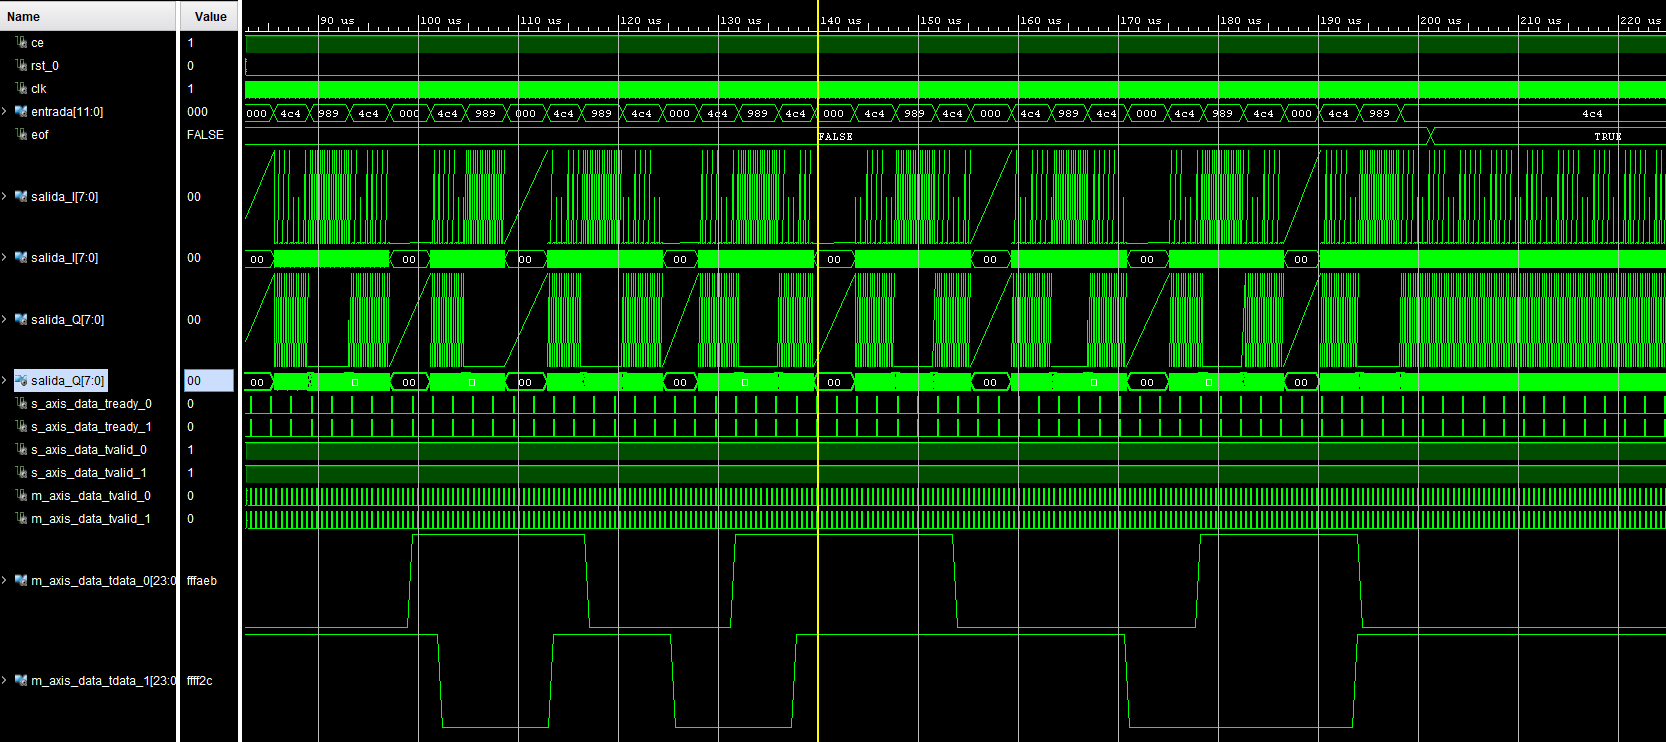
\includegraphics[width=1\textwidth,height=12cm]{img/simu/rrc2.PNG}
	\caption{Simulación de los bloques de mapeado 16-QAM + ZP y filtrado RRC (II)}
	\label{fig:rrc2}
\end{sidewaysfigure}

\chapter{Mezclador de Transmisión}
\label{section:mezcla}

En este Capítulo se describe el último bloque del sistema, correspondiente al mezclador de transmisión. Este bloque se compone de tres procesos: la generación de señales sinusoidales mediante un sintetizador de señal (DDS), la multiplicación de los datos I/Q por estas señales sinusoidales y la suma final de las componentes I/Q de transmisión. En la Figura \ref{fig:mezclador} se visualiza la estructura de los bloques IP que se han incluido en este tercer proyecto de Vivado.

\begin{figure}[h]
    \centering
    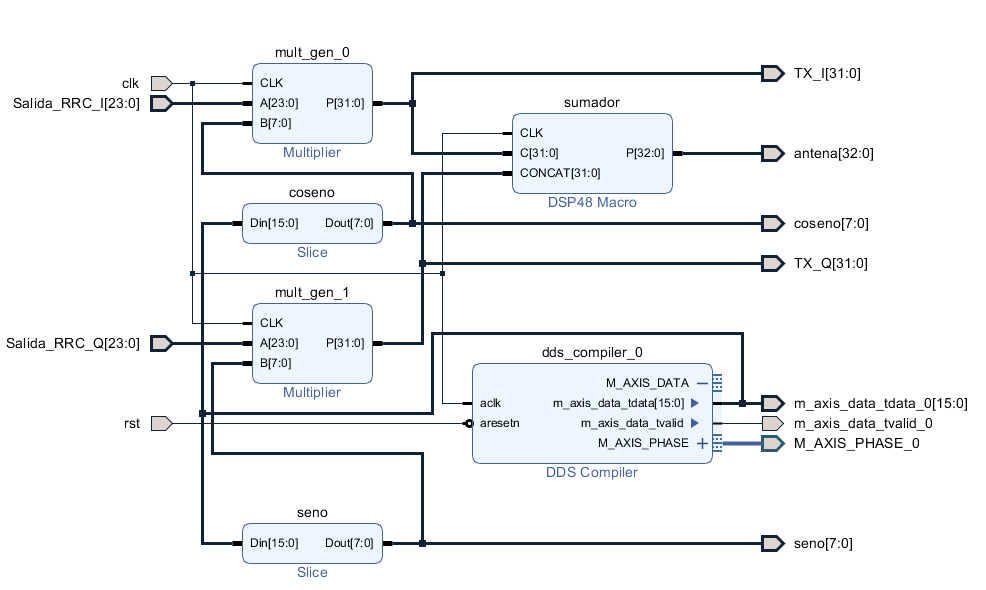
\includegraphics[width=1.05\textwidth, height=10cm]{img/diseno/mezclador.PNG}
    \caption{Diseño del bloque mezclador de transmisión}
    \label{fig:mezclador}
\end{figure}

\pagebreak

\section{Generación de las sinusoides}

Se deben generar dos señales sinusoidales, en particular una función coseno y otra -seno, a partir de un bloque DDS (\textit{Direct Digital Synthesis}). Este bloque es capaz de generar señales analógicas de forma directa mediante un oscilador controlado numéricamente (NCO) y para ello, es preciso configurar internamente la frecuencia de salida deseada de las señales. En el caso de este proyecto será de 100MHz y el reloj del sistema tendrá una frecuencia de 576MHz (3x192MHz), por lo que se obtendrán 5/6 muestras por ciclo.

\vspace{3mm}

La salida del bloque DDS (\textit{m\_axis\_data\_tdata}) esta constituida por 16 bits, de los cuales 8 corresponderán a la señal de seno y los otros 8, a la de coseno como se puede apreciar en la Figura \ref{fig:dds}. Es por ello que se requiere dividir la salida y definir los bits que se dirigirán a la entrada de cada multiplicador mediante dos bloques slice.

\vspace{3mm}

\begin{figure}[h]
    \centering
    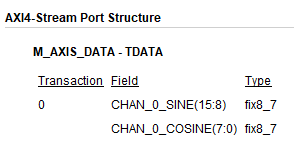
\includegraphics[width=0.45\textwidth]{img/diseno/dds.PNG}
    \caption{Configuración de salida de las señales sinusoidales en el bloque DDS}
    \label{fig:dds}
\end{figure}

\section{Generación de las componentes I/Q y suma}

Para generar las componentes I/Q de transmisión se deben multiplicar las salidas I/Q del filtrado realizado anteriormente por las funciones coseno/-seno generadas en el bloque DDS. Como se ha introducido, el procesamiento de los datos del filtro y el bloque de multiplicación trabajarán a una frecuencia de 576 MHz, siendo el triple de la empleada en los bloques anteriores. 

\vspace{3mm}

Para las salidas I/Q del filtrado (\textit{Salida\_RRC\_I} y \textit{Salida\_RRC\_Q}), es preciso extraer los datos a partir de la lectura de los ficheros \textit{FIR\_output\_I.txt} y \textit{FIR\_output\_Q.txt}, generados anteriormente. A continuación, se muestra el proceso de lectura en el caso de la rama I.

\pagebreak

\begin{lstlisting}[language=VHDL, style=mystyle, caption={Proceso de lectura del fichero de salida del filtrado (rama I)}]
process(clk) 
    --lectura datos salidas filtros
    variable line_buffer : line;
    variable nuevo_valor : integer;
        
    begin
        if rst = '0' then
            eof_I <= false; --se reinicia fin de archivo
        elsif rising_edge(clk) then 
            if not eof_I then
                if endfile(file_handle_I) then 
                    eof_I <= true; 
                elsif m_axis_data_tvalid_0 = '1' then
                    readline(file_handle_I, line_buffer);
                    read(line_buffer, nuevo_valor);
                    Salida_RRC_I <= std_logic_vector(to_signed(nuevo_valor, Salida_RRC_I'length));
                end if;
            end if;
        end if;    
end process;  
\end{lstlisting}

\vspace{3mm}

Como proceso final, se deben combinar las dos componentes I/Q generadas a la salida de los multiplicadores en un bloque sumador. Este se configurará con dos entradas de 32 bits (C y CONCAT) y una salida de 33 bits.


\section{Comprobación de funcionamiento del mezclador}

\begin{lstlisting}[language=VHDL, style=mystyle, caption={Proceso de estimulación}]
process
begin
    file_open(file_handle_I, ".\FIR_output_I.txt", READ_MODE);
    file_open(file_handle_Q, ".\FIR_output_Q.txt", READ_MODE);
  
  
    rst <= '0'; -- negativo
    wait for 100 ns;
    rst <= '1';               

    wait;
end process;
\end{lstlisting}









\chapter{Conclusiones}
\label{section:conclusiones}



%\section{Configuración y uso del bloque MMCM en el diseño}

%Finalmente, se deberá evaluar la eficacia de la modulación 16-QAM en la transmisión de datos
%Se adjunta el enunciado en archivo pdf y un archivo de matlab "qam16.m" para simular el funcionamiento de la transmisión de datos usando 16QAM.

%8.	Codificación de ficheros testbench y pruebas realizadas para la verificación del funcionamiento junto con el simulador Matlab. 
%9. Realización de un diseño modular que funcione correctamente en su conjunto 
%10. Inclusión de otras alternativas/opciones adicionales en el diseño planteado


%Conclusiones:
%Este trabajo se propone como un aporte significativo al entendimiento y aplicación de sistemas de comunicaciones basados en 16-QAM, integrando de manera efectiva los conceptos y tecnologías estudiadas a lo largo de la asignatura. Se espera que los resultados obtenidos contribuyan al desarrollo y mejora continua de sistemas de comunicaciones avanzados.

%===========================================================
%===========================================================

\bibliographystyle{IEEEtran}
\bibliography{refs}


\end{document} 
